\documentclass[format=acmsmall]{acmart}
\begin{document}
\title{GPU-friendly Stroke Expansion}
\author{Raph Levien}
\author{Arman Uguray}
\affiliation{
    \institution{Google}
    \city{San Francisco}
    \state{CA}
    \country{USA}
}

\begin{abstract}
    Vector graphics includes both filled and stroked paths as the main primitives. While there have been many proposed techniques for rendering filled paths on GPU, stroked paths have proved more elusive. This paper presents a technique for performing stroke expansion, namely the generation of an outline representing the stroke of the given input path, an operation which is considered global, but which we nonetheless implement using a fully parallel algorithm. Our method relies on several novel techniques, including an encoding of the input suitable for parallel decoding and processing, an Euler spiral based method for computing flattened parallel curves. While we focus on flattened output consisting of polylines, the methods can be adapted to preserving curves in the output as well.
\end{abstract}

\maketitle
\thispagestyle{empty}
\pagestyle{plain}

\section{Introduction}

Rendering of vector graphics documents requires handling both filled and stroked primitives. There is substantial literature on GPU rendering of filled paths, but many fewer published techniques for strokes. It is a more challenging problem, especially for parallel computation, because path segments cannot be processed independently of each other; the \emph{joins} between adjacent path segments depend on context. In addition, the path topology affects the rendered result, in particular whether subpaths are open or closed. In the former case, the endpoints are rendered with \emph{caps}. Joins and caps can have multiple styles, including different styles within the same document.

The \cite{Nehab2020} paper gives a comprehensive survey of techniques for stroke expansion, and an algorithm which, for a number of reasons, is only suitable for implementation on CPU (though adapting it to GPU is listed as promising future work). It classifies techniques into \emph{local,} where each path segment generates closed geometry (which may be triangles or other primitives), and \emph{global,} where the overall result is a closed outline of the stroked path, but the partial result from each segment is in general open. Our technique is considered global in this scheme, yet allows independent processing of each path segment.

A number of factors contribute to an algorithm being ``GPU-friendly.'' In addition to simply being able to process the input segments in parallel, such an algorithm also avoids divergent control flow (including subdivision for special events such as inflection points and cusps), uses straightforward numerical techniques not subject to particular problems when evaluated using 32-bit floating point numbers.

We propose that the correctness of stroke outlines be divided into \emph{weak correctness} and \emph{strong correctness.} The latter is defined as the computing the outline of a line swept along the segment, maintaining normal orientation, combined with stroke caps and joins. Weak correctness, by contrast, only requires the parallel curves of stroke segments, combined with caps and the outer contours of joins. For sufficiently well-behaved input (particularly when the curvature measured at endpoints of path segements does not exceed the reciprol of the half linewidth), the two notions are equivalent. As described in detail in \cite{Nehab2020}, very few existing implementations actually implement the strong version, so document authors have become accustomed to not depending on behavior at endpoints. Standards for graphics formats also provide an ``out,'' enabling the weaker behavior. [TODO: find language in SVG standard]. While our method emphasizes weak correctness, it likely can be extended to the stronger sense, by implementing evolutes and inner join contours.

\section{Input encoding}

One contribution of this paper is a highly efficient encoding for paths to be rendered. Goals include conciseness, low cost to encode on the CPU side, and fully parallel processing by the GPU. There are two major aspects to the encoding: a variable size encoding of paths, suitable for both filling and stroking, and an extension to stroking. The input is separated into a \emph{tag stream}, with one byte per path element, and another stream for the coordinate data. The index into coordinate data is computed by a prefix sum from a size value derived from the tag byte.

\subsection{Path encoding}

The tag byte is a number of bit fields, packed into a byte.

TODO: make this into a diagram.

\begin{itemize}
    \item 0-1: coordinate count
    \item 2: subpath end bit
    \item 3: 16/32 bit coordinates
    \item 4: path end bit
    \item 5: transform bit
    \item 6: line style bit
\end{itemize}

For most path segments, the coordinate count indicates the type of path segment: 1 for lines, 2 for quadratic Beziers, and 3 for cubic Beziers. The subpath bit is set on the last segment of a subpath, and the path bit is additionally set on the last bit of a path. The latter is not directly interpreted by the path flattening code, but is forwarded to later rendering stages, for example, the path id can be used to select a color or other paint style.

The size is readily inferred from the tag byte: the number of coordinate pairs is the coordinate count plus one if the subpath end bit is set. The nuber of bytes per coordinate pair is 4 for 16 bit coordinates or 8 for 32 bit coordinates.

It is relatively straightforward to convert the standard moveto/lineto/curveto path representation into this encoding. Subpath boundaries are moved from the beginning of a subpath (moveto) to the end. A separate segment must be generated for closepath if the ending point does not coincide with the start point.

The handling of the subpath bit allows for overlap in coordinates, so that, except at subpath boundaries, the first coordinate pair of each path segment overlaps with the last coordinate pair of the previous one. Subpath handling is all computed in the prefix sum; no special handling is needed on the GPU side.

\section{Euler spirals and their parallel curves}

It is common to approximate cubic Béziers to some intermediate curve format more conducive to offsetting and flattening. A number of published solutions (\cite{Yzerman2020}, \cite{Nehab2020}) use quadratic Béziers, as it is well suited for computation of parallel curves. Even so, this curve has some disadvantages. In particular, it cannot model an inflection point, so the source curve must be subdivided at inflection points.

Like these other approaches, we also use an intermediate curve, but our choice is an Euler spiral. In some ways it is similar to quadratic Béziers -- it also has $O(n^4)$ scaling and is best computed using geometric Hermite interpoliation -- but differs in others. It has no difficulty modeling an inflection point. Further, its parallel curve has a particularly simple mathematical definition and clean behavior regarding cusps.

An Euler spiral segment is defined as having curvature linear in arc length.

The parallel curve of the Euler spiral (also known as ``clothoid'') was characterized by Wieleitner well over a hundred years ago\cite{Wieleitner1907}, and has a straightforward closed-form Cesàro representation, curvature as a function of arc length. TODO: present closed-form solution.

\section{Flattened parallel curves}

The geometry of a stroke outline consists of joins, caps, and the two parallel curves on either side of the input path segemnts, offset by the half linewidth. The former are not particularly difficult to calculate, but parallel curves of cubic Béziers are notoriously tricky. Analytically, is is a tenth order algebraic curve, which is not particularly feasible to compute directly.

Conceptually, generating a flattened stroke outline consists of computing the parallel curve of the input curve segment followed by \emph{flattening,} the generation of a polyline that approximates the parallel curve with sufficient accuracy (which can be measured as Fréchet distance). However, these two stages can be fused for additional performance, obviating the need to store a representation of the intermediate curve.

Using a subpixel Fréchet distance bound guarantees that the rendered image does not deviate visibly from the exact rendering. Another choice would be uniform steps in tangent angle, as chosen by \cite{Kilgard2020}. However, at small curvature, the stroked path can be off by several pixels, and at large curvature there may be considerably more subdivision than needed for faithful rendering.

Proposed image: show circular arcs with polar stroking vs near-optimal flattening.

\subsection{Optimal flattening}

The optimal flattening of a curve, with a maximum error constraint, is as follows. An optimal flattening contains the minimum number of subdivisions required to meet that constraint. Further, the error is the minimum possible with that number of subdivisions.

For a convex curve, the optimal flattening is tractable to compute, though not necessarily very fast. When a curve is monotonic, error is also monotonic with respect to both subdivision points. Thus, any standard root finding technique can find a subdivision with a given error (bisection is the best known, but the ITP method \cite{Oliveira2020} is better). An similar outer loop with a root finding technique can find the error which minimizes the global error for the entire flattening, which, due to monotonicity, is that for which the error of the final segment equals that of the previous segments. Subdividing at the inflection point adds at most one additional point; it is possible to optimize further, but we do not consider that (though the near-optimal flattening we will later present is not subject to this constraint).

\subsection{Density-based subdivision}

It is possible to analytically determine the optimal subdivision in the limit as the error approaches zero. Considering the local region of a curve as having constant curvature $\kappa$, when the distance between two subdivision points is $\Delta x$, the error is $\frac{1}{2}\Delta x^2 \kappa$. Thus, in the continuous limit, the number of subdivision points per unit length is $\sqrt{\frac{\kappa}{2\Delta y}}$, where $\Delta y$ is the target error tolerance. We call $\sqrt{\kappa}$ the \emph{subdivision density}, and scaling it by $\frac{1}{\sqrt{2\Delta y}}$ (which is constant for the curve) yields the number of subdivision points per unit length.

Sampling the curvature at a point is problematic. At an inflection point, the curvature is zero, indicating that no subdivision is needed. Conversely, at a cusp, curvature is infinite, so a technique based on sampling the curvature and advancing by the amount predicted by a circular arc at the sample point would fail to advance (the sampling density would be infinite at that point). In both cases, the sampling density varies along the curve.

Our solution is, instead of \emph{sampling} the subdivision density to determine a subdivision interval, we instead compute its \emph{integral.} Since the sampling density is in subdivisions per unit length (after proper scaling to take into account the error tolerance), the integral over the arc length between two subdivision points should be one. Computing the integral over the length of the curve segments gives the number of subdivisions needed. Rounding up, then dividing that quantity evenly by the number of subdivisions, then computing the inverse integral, gives the location of subdivision points in a nearly optimal flattening.

The integral is expressed over arc length, but for convenience and efficient computation can be re-parametrized as desired. For computing the parallel curve of an Euler spiral, the natural parametrization is the arc length of the source curve. In this case, the conversion between the two is a simple (and readily invertible) equation, as given by \cite{Wieleitner1907}, but even that is not necessary in general; by computing the integral, and its inverse, in terms of the convenient parametrization, no explicit conversion to or from arc length is needed.

\subsection{The subdivision density integral}

The subdivision density for an Euler spiral, normalized so that its inflection point is at -1 and the cusp of the parallel curve is at 1, is simply $1 - \sqrt{|1-s^2|}$. This function is plotted in Figure\ref{fig:subdiv_density}.

\begin{figure}
    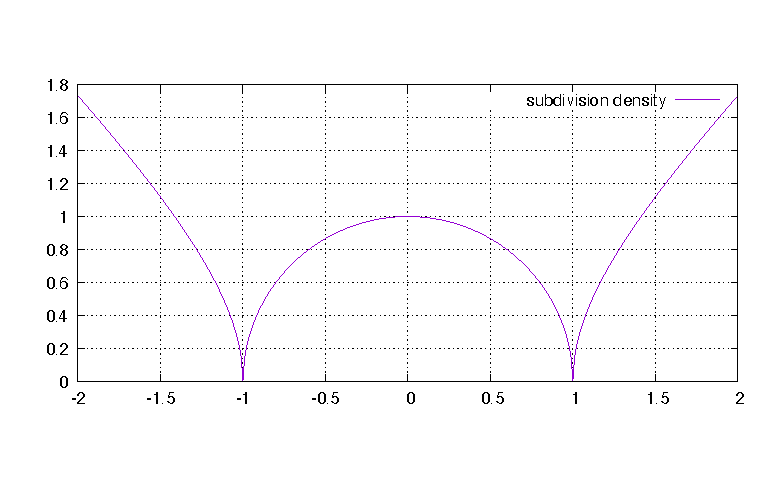
\includegraphics{subdiv_density}
    \caption{Subdivision density for the parallel curve of an Euler spiral}
    \Description{A graph of subdivision density. The range from -1 to 1 is a semicircle, and the value from 1 rises sharply from zero to an asymptote of unity slope.}
    \label{fig:subdiv_density}
\end{figure}

The subdivision density integral for the parallel curve of an Euler spiral is given as follows:

\[
    f(x) = \int_0^x\sqrt{|u^2 - 1|} du
\]

This integral has a closed-form analytic solution:

\[
    f(x) = \left\{
        \begin{array}{rl}
            \frac{1}{2}(x\sqrt{|x^2-1|} + \sin^{-1}x) & \text{if } |x| \leq 1 \\
            \frac{1}{2}(x\sqrt{|x^2-1|} - \cosh^{-1}x + \frac{\pi}{4} & \text{if } x \geq 1
        \end{array}
    \right.
\]

Values for $x<-1$ follow from the odd symmetry of the function. 


\subsection{Approximation of the subdivision density integral}

The subdivision density integral [TODO: probably should use section or equation number reference] is fairly straightforward to compute in the forward direction, but not invertible using a straightforward closed-form equation. Numerical techniques are possible, but require multiple iterations to achieve sufficient accuracy, so are slower. In this subsection, we present a straightforward and accurate approximation, based on piecewise easily invertible functions. If higher flattening quality is desired at the expense of slower computation, this approximation can be used to determine a good initial value for numeric techniques; two iterations of Newton solving are enough to refine this guess to within 32-bit floating point accuracy.

The approximation is given as follows:

\[ 
    f_\mathit{approx}(x) = \left\{
        \begin{array}{rl}
            \frac{\sin c_1 x}{c_1} & \text{if } x < 0.8 \\
            \frac{\sqrt{8}}{3}(x-1)^{1.5} + \frac{\pi}{4} & \text{if } 0.8 \leq x < 1.25 \\
            0.6406x^2 - 0.81x + c_2 & \text{if } 1.25 \leq x < 2.1 \\
            0.5x^2 - 0.156x + c_3 & \text{if } x \geq 2.1
        \end{array}
        \right.
\]
\[
    \begin{array}{ll}
        c_1 = & 1.0976991822760038 \\
        c_2 = & 0.9148117935952064 \\
        c_3 = & 0.16145779359520596
    \end{array}
\]

The primary rationale for the constants is for the approximation to be continuous. The other parameters were determined empirically; further automated optimization is possible but is unlikely to result in dramatic improvement. Further, this approximation is given for positive values. Negative values follow by symmetry, as the function is odd.

The exact integral and the approximation given above are shown in Figure~\ref{fig:espc}. Visually, it is clear that the agreement is close, and in numerical testing the worst case discrepancy between approximate and exact results is approximately 6\%.

\begin{figure}
    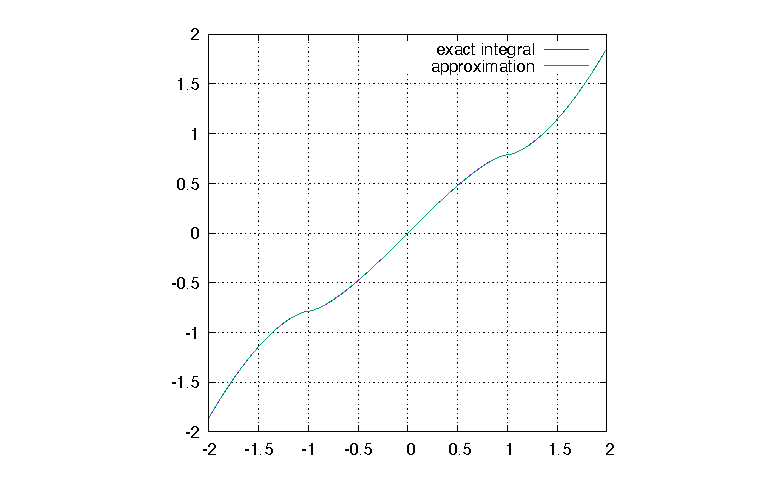
\includegraphics{espc}
    \caption{Integral of subdivision density for Euler spiral parallel curve, and its approximation}
    \Description{A graph of the integral of subdivision density. It is a wriggly diagonal line, with flat parts at -1 and 1. The approximation is nearly indistinguishable from the exact value.}
    \label{fig:espc}
\end{figure}

\section{Evolutes}

In the principled, correct specification for stroking\cite{Nehab2020}, parallel curves are sufficient only for segments in which the curvature does not exceed the reciprocal half width. When it does, additional segments must be drawn, including evolutes of the original curve. In general, the evolute of a cubic Bézier is a very complex curve, requiring approximation techniques. By contrast, the evolute of an Euler spiral ($\kappa = as$) is another spiral with a simple Cesàro equation, namely $\kappa = -a^{-1}s^{-3}$, an instance of the general result that the evolute of a log-aesthetic curve is another log-aesthetic curve\cite{Yoshida2012}.

Flattening this evolute is also straightforward; the subdivision density is proportional to $s^{-0.5}$ where $s$ is the arc length parameter of the underlying Euler spiral (and translated so $s = 0$ is the inflection point). Thus, the integral is $2\sqrt{s}$, and the inverse integral is just squaring. Thus, flattening the evolute of an Euler spiral is simpler than flattening its parallel curve.

TODO: figure showing ES, its evolute, and subdivision points for flattening.

\section{Conversion from cubic Béziers to Euler spirals}

The Euler spiral segment representation of a curve is useful for computing near-optimal flattened parallel curves, but standard APIs and document formats overwhelmingly prefer cubic Béziers as the path representation.

Many techniques for stroke expansion described in the literature apply some lowering of cubic Bézier curves to a simpler curve type, more tractable for evaluating parallel curve. Computing parallel curves directly on cubic Bézier curve segments is not very tractable. In particular, the widely cited Tiller-Hanson algorithm\cite{Tiller1984} performs well for quadratic Béziers but significantly worse for cubics.

A typical pattern for converting from one curve type to another is \emph{adaptive subdivision.} (TODO: is there a good general reference for this?) An approximate curve is found in the parameter space of the target curve family. The error of the approximation is measured. If the error exceeds the specified tolerance, the curve is subdivided (typically at $t = 0.5$), otherwise the approximation is accepted. Subdivisions are also indicated at special points; for example, since quadratic Béziers cannot represent inflection points, and geometric Hermite interpolation is numerically unstable if the input curve is not convex, lowering to quadratic Béziers also requires calculation of inflection points and subdividing there. A good example of this pattern is Nehab\cite{Nehab2020}. One advantage of Euler spirals over quadratic Béziers is that they can represent inflection points just fine, so it is not necessary to compute those for additional subdivision.

The approach in this paper is another variant of adaptive subdivision, with two twists. First, it's not necessary to actually generate the approximate curve to measure the error. Rather, a straightforward closed-form formula accurately predicts it. The second twist is that, since compute shader languages on GPUs typically don't support recursion, the stack is represented explicitly and the conceptual recursion is represented as iterative control flow. This is an entirely standard technique, but with a clever encoding the entire state of the stack can be represented in two words, each level of the stack requiring a mere single bit.

\subsection{Error prediction}

TODO: provide formula: area, halo, center

\subsection{Geometric Hermite interpolation}

Given tangent angles relative to the chord, finding the Euler spiral segment that minimizes total curvature variation is a form of geometric Hermite interpolation. There are a number of published solutions to this problem, all involving nontrivial numerical solving techniques: gradient descent\cite{Kimia2003}, bisection\cite{Walton2009}, or Newton iteration\cite{Connor2014}. Our approach is much more direct. We observe that the Euler spiral parameters are a smooth function of the two input parameters, and determine a 2D Taylor's series for this function. Many of the terms are zero because of symmetry. Preserving terms up to 7th order provides excellent accuracy (TODO: quantify more carefully) with modest computational expense.

TODO: the technique used is a refinement of what was sketched in the Python notebook attached to the "cleaner parallel curves with Euler spirals" blog post. It's basically a 2D Taylor's series. Previously we had the secant method from section 8.2 of my thesis; not sure whether we want to cite that in the submission for anonymity reasons. It's functionally pretty similar to the \cite{Connor2014} reference.

\subsection{Unrolled recursion}

The entire recursion stack for adaptive subdivision can be represented in two words: dt and scaled\_t0. The range is dt * scaled\_t0 .. dt * (scaled\_t0 + 1). Initial values of 1 and 0 represent the range (0, 1). Pushing the stack, subdividing the range in half, is representing by halving dt and doubling scaled\_t0, which leaves the start of the range invariant but its size halved. After accepting an approximation, the next range is determined by incrementing scaled\_t0, then repeatedly popping the stack by doubling dt and halving scaled\_t0, as long as the latter is odd. This can in fact be achieved without iteration by using the "count trailing zeros" intrinsic.

\section{Discussion}

\bibliographystyle{ACM-Reference-Format}
\bibliography{paper}

\end{document}
